\subsection{Global Interconnect Networks}

Ever since the introduction of the first international mobile communication standard \gls{gls:2g}/GSM, \glspl{mno} around the world exchange signaling and user data via the global \gls{ipx} network.
Designed to be a private channel for communication amongst \glspl{mno} only, the way in which it is used today, and the plethora of different parties connected to it --many of them not network operators-- renders it a network that is not any more trustworthy than the public Internet.
Coupled with weaknesses in the established network protocols as previously summarized in section~\ref{sec:related}, the interconnect interface is cause for major security and fraud concerns for any mobile service provider.

One of the reasons why this well-known problem still persists several years after the publication of possible exploits is the role that operators of \gls{ipx} peering platforms play in inter-\gls{plmn} signaling, which goes well beyond that of pure connectivity providers.
Many \glspl{mno} depend on them for supplementary services that require accessing or even modifying the contents of signaling traffic.
These services include, for example, normalization of the protocol syntax, replacement of attributes to alleviate technical incompatibilities, and business intelligence offerings.
Note, that for the communication partners on either side it is intransparent which routing path messages take on the interconnect network.
A single \gls{plmn} can simultaneously be connected to multiple \gls{ipx} providers, which in turn may or may not connect directly to each other.
\gls{3gpp} assumes a model in which there is at least one or more \gls{ipx} provider in any given routing path (see \cite{3gpp.33.501}, p.~130):

\begin{enumerate}[label=--]
    \item Both \glspl{plmn} are connected to the same \gls{ipx} provider that is allowed to access message contents.

    \item Both \glspl{plmn} are connected to two distinct \gls{ipx} providers that are each allowed to access message contents and that are connected directly to each other.

    \item Both \glspl{plmn} are connected to two distinct \gls{ipx} providers that are each allowed to access message contents and that are connected via additional \gls{ipx} providers not expected to access message contents.
\end{enumerate}

As \gls{plmn} operators have a business relationship with their directly connected \gls{ipx} providers, these entities are considered trusted to the extend that they may supply modifications to incoming and outgoing messages.
Similarly, the \gls{ipx} provider directly connected to the peer operator is trusted by extension, as both \glspl{mno} have a business relationship between each other governing the allowed message modifications.
Lastly, third-party \gls{ipx} providers in between the ones directly connected to either of the mobile networks should not modify any message components or access confidential information.

Intuitively, one can dicern an overlap with the premises of the Dolev-Yao model:
All signaling messages are intercepted or potentially blocked by an \gls{ipx} provider, i.e. the potential adversary, and all messages received by any mobile network operator are sent by such an entity.
This constellation, in which different external parties are expected to perform certain changes that cannot be validated or traced with existing security protocols is one of the motivating factors for the definition of \gls{prins}.
It is supposed to provide the technical controls to enforce the trust model outlined above.

\subsection{5G Core Network Signaling}

\begin{wrapfigure}{r}{0.30\textwidth}
    \begin{center}
    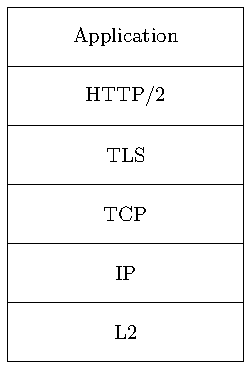
\includegraphics[width=0.25\textwidth]{n32-stack.pdf}
    \end{center}
    \caption{5G control plane stack, according to TS 29.573 (\cite{3gpp.29.573}, p.~11)}
    \label{fig:5g-stack}
\end{wrapfigure}

\gls{3gpp} Release 15 features a redesigned protocol stack for communication between 5G \gls{gls:cn} functions, illustrated in figure \ref{fig:5g-stack}.
Rather than relying on specialized protocols that are almost exclusively used in previous generations of mobile networks, 5G makes broad use of protocols, formats, and principles popular in the domain of web services.
It is important to note that the 5G \gls{gls:up} is exempt from these changes and is still relying on the same protocols as in 4G/LTE.
The 5G \gls{gls:cp} however, has been updated as follows.
The \gls{tcp} is used on transport layer, rather than the \gls{sctp}.
On top of that, \gls{ip} packets carry \gls{http}/2 messages that may optionally be protected by \gls{tls}.
Inside the \gls{http} body additional information structured as \gls{json} objects can be transferred.
Communication between 5G Core \glspl{nf} evolves around standardized \glspl{api} that are modeled according the principles of \gls{rest}.
This design decision brings with it a number of constrains originally layed out by \cite{fielding2000arch}.
The ones adopted by \gls{3gpp} in Release 15 are summarized below (see~\cite{mayer2018restful}, p.~109-114):

\begin{enumerate}[label=\arabic*), wide, labelwidth=!, labelindent=0pt]
    \item \textit{Resources, Resource Identifiers, and Resource Representation}

    \noindent
    Every single data point that might be the target of a signaling message is considered a resource.
    A resource is an abstract entity that may be referenced by identifiers.
    Its information can be conveyed in varying representations, e.g. a \gls{json} object.

    \item \textit{Client-Server Communication}

    \noindent
    Communication follows a strict separation of concerns, allowing both client and server to evolve independently as long as the defined \glspl{api} are used.
    In the \gls{3gpp} specification the terms consuming \gls{nf} and producing \gls{nf} are equally used.

    \item \textit{Statelessness}

    \noindent
    Signaling messages are expected to be completely self-contained, allowing the receiving party to intepret them without any additional state information stored across multiple requests/responses.
    Although this holds true for \gls{http} itself, both \gls{tls} and \gls{prins} being stateful protocols do not adhere to this constraint.

    \item \textit{Cache}

    \noindent
    Resulting from item 3) is the ability of the client or intermediaries to store certain responses temporarily for future (re-)use.
    A possible way to optimize intra-\gls{plmn} signaling latency, this behaviour is not relevant for inter-operator communication.

    \item \textit{Layered Systems}

    \noindent
    This constraint demands that the client does not need to be aware of what exactly happens on server side to fulfill a request or even what server instance is answering.
    In essence, this is about decoupling of individual services which is inherent to the design of the 5G \gls{gls:cn}.

\end{enumerate}

The above-mentioned changes to the protocol stack also extend to the signaling channel between \glspl{plmn}, i.e. the N32 interface.
But aside from modernizing the protocols, a redesigned \gls{gls:cn} architecture entails further improvements to enhance interconnect security.
Whereas earlier mobile generations only specify protection on the transport layer by means of IPsec, which in practice is rarely used due to operator requirements cited in the previous section, 5G aims to offer more flexible protection on application layer.
For this purpose, a dedicated Network Function is introduced to ensure security on the N32 interface.
The \gls{sepp} is tasked with applying confidentiality and integrity protection to outbound signaling messages, depending on operator-controlled protection policies.
Simultaneously, it is the single point of contact for all inbound signaling traffic, ensuring mutual authentication with all peer \glspl{sepp}, enforcing message integrity, rate limits, and further security checks.
A complete list of \gls{sepp} requirements is given in TS 33.501 (\cite{3gpp.33.501}, p.~31).

When an \gls{nf} needs to exchange \gls{gls:cp} messages with an entity in a different \gls{plmn}, it addresses the \gls{sepp} in its own network.
The \gls{sepp} transforms the complete \gls{http} message into a \gls{json} object before applying security on the individual information elements contained.
Protection is provided by means of \gls{jwe} and symmetric keys shared between peer \glspl{sepp}.
Afterwards, the transformed message sent on the N32 interface towards the roaming partner's \gls{sepp} via one or more \gls{ipx} providers.
Authorized \gls{ipx} providers may add changes to the transported messages, using the \gls{json} patch method specified in RFC 6902  (\cite{rfc6902}).
Each patch is digitally signed using \gls{jws} and the \gls{ipx} provider's private key.
Before any message modifications are possible, the related public key needs to be shared with the involved \glspl{mno}.
By relying on asymmetric cryptography, traceability of any intermediary patches can be ensured.
Once a \gls{sepp} receives an incoming message on the N32 interface, it validates the integrity of the original contents and any patches added by \gls{ipx} providers.
If this validation is successful, the added \gls{json} patches originate from authorized sources and only modify information elements that are allowed to be accessed, the \gls{sepp} transforms the \gls{json} element back into a signaling message, applying changes by the \gls{ipx} providers in the process.
The resulting \gls{http} message is forwarded to the destination \gls{nf}.
This flow is illustrated in figure \ref{fig:n32} below.

\begin{figure}[ht!]
    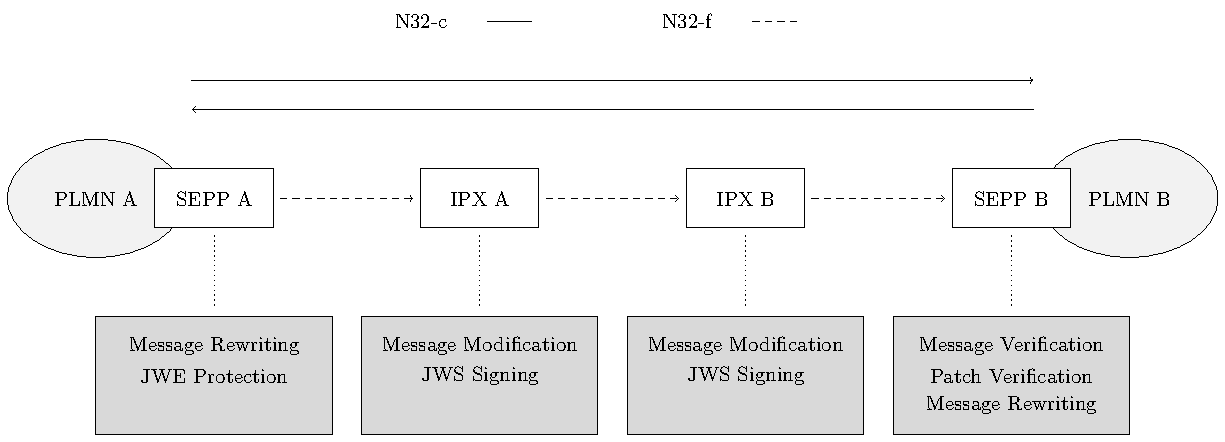
\includegraphics[width=\textwidth]{n32-interface.pdf}
    \centering
    \caption{5G interconnect architecture, according to TS 33.501 (\cite{3gpp.33.501}, p.~131)}
    \label{fig:n32}
\end{figure}

\subsection{PRINS Protocol Structure}
\label{ssec:prins-structure}
\subsubsection{Protocol Channels}

The 5G inter-operator signaling protocol provides security for messages on the N32 interface between two \glspl{sepp}.
The protocol is comprised of two logical channels.\medskip

\textbf{N32-c} is a \gls{tls}-protected connection used for session management.
Once an interconnect session is established, each of the communicating \glspl{sepp} sets up an N32-c channel to be able to send and receive related messages by its peer.
Information exchanged via this channel serve the purpose of session parameter exchange (e.g. protection policies and cryptographic profiles), error handling throughout the communication, as well as session termination.
Since none of these use cases require access to the message contents by any intermediaries, messages are transported via this dedicated end-to-end protected channel.

If none of the operators on either end of the communication have a need for the active involvement of \gls{ipx} providers, \gls{3gpp} also specifies the option to utilize the N32-c channel directly for transfering signaling messages without the use of \gls{prins}.
This purely \gls{tls}-based operation is mentioned only for completeness sake and shall not be analyzed in detail.\medskip

\textbf{N32-f} is a \gls{prins}-protected connection carrying \gls{http} messages that contain the inter-operator signaling data serialized into \gls{json} objects.
The level of protection provided for individual information elements in these messages is determined by two types of protection policies, specified by the communicating parties:

\begin{enumerate}[label=--]
    \item \textit{Data-type encryption policy}, describing what types of information elements require confidentiality protection.
    \item \textit{Modification policy}, describing what information elements are allowed to be modified by intermediaries \gls{ipx} providers.
\end{enumerate}

The data-type encryption policy is supported by an \textit{\gls{nf} \gls{api} data-type placement mapping}, defining the data-type of a particular information element.
The \gls{prins} protocol expects this policy to be the same in both communicating \glspl{sepp} in order to rule out inconsistencies in confidentiality requirements:
,,The data-type encryption policies in the two partner SEPPs shall be equal to enforce a consistent ciphering [...]'' (\cite{3gpp.33.501}, p.~135).
In addition to the operator-defined data-type encryption policies, \gls{3gpp} defines a set of data-types to be confidentiality protected mandatorily.
That is, data of type ,,Authentication Vectors'', ,,Location data'', and ,,Cryptographic material'' (\cite{3gpp.33.501}, p.~31).
None of the custom protection policies compiled by the operators should contradict these default protection requirements.
However, the specification does not describe how a potential misconfiguration is to be handled by either of the \glspl{sepp}.

The modification policy of each communicating party is only applicable to the \gls{ipx} provider that the defining \gls{mno} has a business relationship with, i.e. any mobile network operator can only actively allow changes by its directly connected interconnection providers.
By default, any modifications by intermediaries are prohibited.
The policy is roaming partner specific, i.e. one needs to be defined peer \gls{plmn}/\gls{ipx} provider combination.
\\

An N32-f session is identified by an \textit{N32-f context} -- supplementary session information stored by each \gls{sepp} in order to correlate and validate related messages.
This information can be summarized as follows:

\begin{enumerate}[label=--]
    \item \textit{N32-f context ID}, uniquely identifying a given N32-f session.
    \item \textit{N32-f peer information}, containing the peer \gls{plmn} ID, peer \gls{sepp} ID, and its \gls{ip} address.
    \item \textit{N32-f context information}, containing details on session validity and an indication whether to use \gls{prins} or \gls{tls}.
    \item \textit{N32-f security context}, including the \gls{prins} session keys, \gls{jose} cipher suites, protection policies, session counters, initialization vectors, and a so-called \gls{ipx} security information list.
\end{enumerate}

The N32-f context ID is created by both \glspl{sepp} during the initial handshake procedure described in the following subsection.
It is referenced in each N32-f message in order to inform the receiving \gls{sepp} which session to correlate it to.

The N32-f peer information holds the \gls{plmn} ID and an additional \gls{sepp} ID in order to differentiate multiple instances in the foreign network.
A remote \gls{sepp} address is required for routing purposes.

The N32-f security context further references the aforementioned protection policies, as their scope is one particular N32-f session.
The agreed cryptographic algorithms for \gls{jwe} protection are stored as cipher suites.
Lastly, the N32-f security context holds an \gls{ipx} security information list -- identifiers of all intermediary \gls{ipx} providers as well as the related  public keys or certificates used to validate message modifications submitted by them.
If certificates are being used, it is expected that \glspl{mno} act as certificate authorities for their IPX providers, issuing certificates for them to sign their message modifications.

Also contained in the N32-f security context is the N32-f key hierarchy, which is comprised of a single master key generated from the initial N32-c \gls{tls} session, using the \gls{tls} export mechanism specified in RFC 5705 (\cite{rfc5705}), as well as two sets of session keys and \gls{iv} derived form the master key and sequence counters.
The latter are used for applying \gls{jwe} protection to N32-f messages -- keys for encryption, \glspl{iv} and counters for constructing the nonce required by \gls{aes}-\gls{gcm}.
Two sets of each are required since N32-f, similar to N32-c, requires setting up two distinct \gls{http} connections to enable a \gls{sepp} to both send and receive messages.
Hence, \gls{3gpp} specifies \textit{parallel} session keys and \glspl{iv} for use by the \gls{sepp} that initialted the N32-c session.
The other sets of \textit{reverse} session keys and \glspl{iv} are to be used for a \gls{prins} session with the \gls{sepp} that responded to the initial N32-c establishment (see~\cite{3gpp.33.501}, p.~141-142):
\\

\begin{minipage}[l]{0.5\textwidth}
    \begin{enumerate}[label=--]
        \item \texttt{parallel\_request\_key}
        \item \texttt{parallel\_response\_key}
        \item \texttt{parallel\_request\_iv\_salt}
        \item \texttt{parallel\_response\_iv\_salt}
    \end{enumerate}
\end{minipage}%
\begin{minipage}[r]{0.5\textwidth}
    \begin{enumerate}[label=--]
        \item \texttt{reverse\_request\_key}
        \item \texttt{reverse\_response\_key}
        \item \texttt{reverse\_request\_iv\_salt}
        \item \texttt{reverse\_response\_iv\_salt}
    \end{enumerate}
\end{minipage}\medskip

\subsubsection{N32-f Message Format}

Signaling messages sent towards receivers in a different \gls{plmn} are reformatted into a \gls{json} structure by the \gls{sepp} before being forwarded on the N32 interface.
Depending on the protection requirements described in the configured policies, individual parts of the original \gls{http} message are placed in different locations.
\gls{3gpp} defines two objects to be created by the sending \gls{sepp}.
An overview of the complete message structure is provided in figure \ref{fig:n32f-message}.

\begin{enumerate}[label=--]
    \item \textit{dataToIntegrityProtect} holds all information to be integrity protected.
    This includes the complete messages with all its \gls{http} headers, pseudo-headers (e.g. \gls{http} method), and the \gls{http} message body with the exception of information elements requiring confidentiality protection, whose values are replaced by null.
    The \gls{sepp} further supplies additional N32-f specific meta data, i.e. N32-f message ID, N32-f context ID, and an ID of the directly connected \gls{ipx} provider.

    \item \textit{dataToIntegrityProtectAndCipher} contains information to be both integrity and confidentiality protected.
    The \gls{sepp} creates a \gls{json} patch for each of the concerned elements of the original message and such that there is a patch replacing each of the null values in the \textit{dataToIntegrityProtect} object.
\end{enumerate}

Following the reformatting, both of these \gls{json} objects are protected using \gls{jwe}.
For this purpose, \gls{3gpp} only specifies encryption methods that build on \gls{aead}, i.e. cryptographic schemes ensuring both confidentiality and authenticity of data.
The use of \gls{jwe} with these particular cipher suites allows for the choice to protect integrity and confidentiality of certain objects while others are only integrity protected.
Resulting from this operation is the ciphertext itself and a \gls{jwe} authentication tag, which can be used to verify the integrity of both the ciphertext and the \gls{aad}.

IPX providers performing intermediate changes are only allowed to do so on the clear text parts of the N32-f message, i.e. the \textit{dataToIntegrityProtect} object.
Modifications are not applied directly, but appended to the original message as a separate \gls{json} patch.
Before forwarding the message to the next hop, the complete \textit{modifiedDataToIntegrityProtect} object is signed using \gls{jws} and the private key belonging to the IPX provider's certificate issues by its client \gls{mno}.

\begin{enumerate}[label=--]
    \item \textit{modifiedDataToIntegrityProtect} contains the operations to be performed on the original message's \textit{dataToIntegrityProtect} object. In addition, the IPX provider supplies a unique identity that is not further defined. Lastly, the \gls{jwe} authentication tag created by the sending \gls{sepp} is included as well, serving the purpose of replay protection.
\end{enumerate}

\begin{figure}[h!]
    \centering
    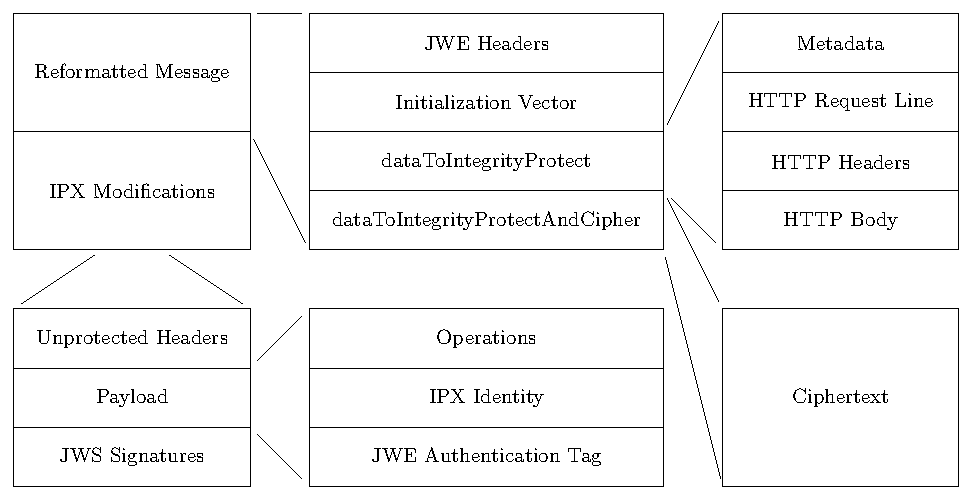
\includegraphics[width=\textwidth]{n32f-message.pdf}
    \caption{N32-f message structure according to TS 29.573 (\cite{3gpp.29.573}, p.~21)}
    \label{fig:n32f-message}
\end{figure}

\subsection{PRINS Sequences and Security Properties}
\label{ssec:prins-sequence}

Following the individual components of the \gls{prins} protocol, the following section provides a step-by-step description of the complete N32-c and N32-f message flows as specified in TS 33.501 (see \cite{3gpp.33.501}, pp.~129, 141-143).
In preparation of the formal verification in chapter~\ref{chap:verification}, the protocol's intended security properties are specifically highlighted.
It should be noted that \gls{3gpp} specifications, being written in an informal style, may not explicitly spell out all security requirements to be met by the \gls{prins} protocol.
Therefore, a distinction is made between security properties which are explicitly cited in the document (hereafter highlighted in blue) and those that can be derived implicitly from the its contents (hereafter highlighted in gray).

\begin{minipage}{0.5\textwidth}
    \sgoal{
        Explicitly defined\newline security property
    }
\end{minipage}
\begin{minipage}{0.4\textwidth}
    \asgoal{
        Implicitly defined\newline security property
    }
\end{minipage}

\subsubsection{N32-c}

\begin{figure}[h!]
    \centering
    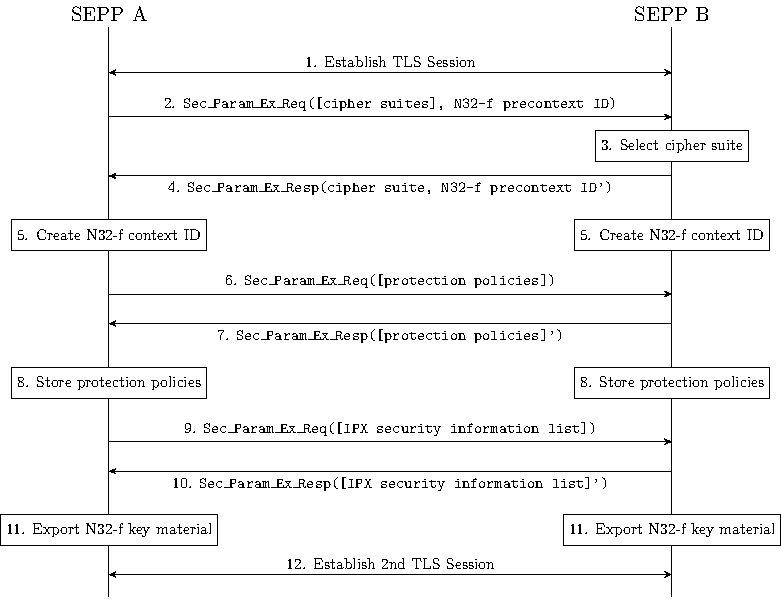
\includegraphics[width=\textwidth]{n32c-flow.pdf}
    \caption{N32-c Sequence Diagram}
    \label{fig:n32c-sequence}
\end{figure}

\begin{enumerate}[wide, labelwidth=!, labelindent=0pt]
    \item Initially, two peer \glspl{sepp} establish an end-to-end protected \gls{tls} session on the basis of the previously exchanged raw public keys or certificates for authentication.
    \asgoal{
        Security property 1: N32-c sessions between two \glspl{sepp} shall be mutually authenticated.
    }
    \asgoal{
        Security property 2: Information exchanged in an N32-c session shall be confidentiality protected and integrity protected.
    }
    \item The initiating \gls{sepp} sends an ordered list of supported \gls{jose} cipher suites and its N32-f precontext ID in a \texttt{Security\_Parameter\_Exchange\_Request} to its peer.
    \item The responding \gls{sepp} selects one of the provided cipher suites based on its locally configured priority.
    \item The responding \gls{sepp} answers the preceding message with a \texttt{Security\_Parameter\_} \texttt{Exchange\_Response} containing the highest priority cipher suite supported by both \glspl{sepp} and its own N32-f precontext ID.
    \item Both \glspl{sepp} create the final N32-f context ID by concatenating the initiating \gls{sepp}'s precontext ID with the the responding \gls{sepp}'s precontext ID, in that order.
    \asgoal{
        Security property 3: Following above step 5, both \glspl{sepp} shall agree on the same N32-f context ID value.
    }
    \item The initiating \gls{sepp} may send its protection policies to its peer. Alternatively, both data-type encryption policies and modicifation policies can also be preconfigured manually.
    \item Similarly, the responding \gls{sepp} may send its own protection policies as well.
    \item If one of the \glspl{sepp} exchanged its protection policies in the previous stops, the counterparty shall store these policies in its N32-f security context.
    \item The initiating \gls{sepp} sends the \gls{ipx} security information list to its peer. This list contains information about the \gls{ipx} provider(s) the \gls{sepp}'s operator has authorized to perform message modifications.
    \item Equally, the same information about the IPX provider(s) authorized by the responding \gls{sepp}'s operator are provided in the opposite direction.
    \item Both \glspl{sepp} use the TLS export function to derive pseudo-random key material for the N32-f session.
    \asgoal{
        Security property 4: Following above step 11, both \glspl{sepp} shall derive the same N32-f master key.
    }
    \item The responding \gls{sepp} creates a separate \gls{tls}-protected N32-c session, enabling it to actively send messages to the initiating \gls{sepp}. Both \glspl{sepp} leave their N32-c channels open throughout the complete lifetime of a session for the purposes of secure error signaling and session management.
    \asgoal{
        Security property 5: An adversary shall not be able to detect a change in session keys.
    }
\end{enumerate}

\subsubsection{N32-f}

\begin{figure}[h!]
    \centering
    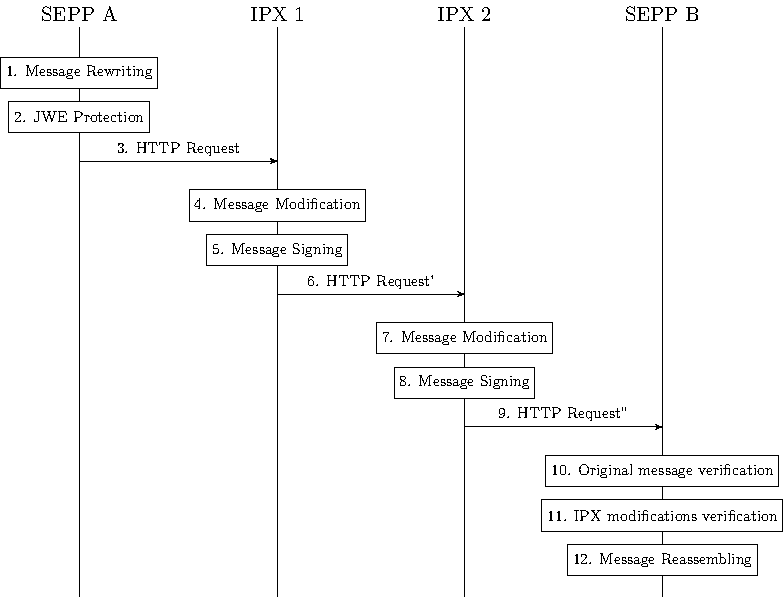
\includegraphics[width=\textwidth]{n32f-flow.pdf}
    \caption{N32-f Sequence Diagram}
    \label{fig:n32f-sequence}
\end{figure}

\begin{enumerate}[wide, labelwidth=!, labelindent=0pt]
    \item After receiving a signaling message from an \gls{nf} in its network, the sending \gls{sepp} rewrites the message into the \gls{json} structures described previously.
    \item On the resulting object, the sending \gls{sepp} applies \gls{jose} protection as follows: The \textit{dataToIntegrityProtectAndCipher} object serves as input to be ciphered, whereas the \textit{dataToIntegrityProtect} object is used as \gls{aad}.
    \sgoal{
        Security property 6: Information in the \textit{dataToIntegrityProtect} object shall be integrity protected. (c.f. \cite{3gpp.33.501}, p.~138)
    }
    \sgoal{
        Security property 7: Information in the \textit{dataToIntegrityProtectAndCipher} object shall be confidentiality and integrity protected. (c.f. \cite{3gpp.33.501}, p.~138)
    }
    \item The protected \gls{json} object is embedded into the body of a new \gls{http} request and sent to the first \gls{ipx} provider.
    \item The first \gls{ipx} provider in the path parses the \textit{dataToIntegrityProtect} object and determines the necessary changes. It creates a new \textit{modifiedDataToIntegrityProtect} object, containing a list of all modifications. If there are no modifications to be performed, the \gls{ipx} provider shall write the empty list into the \textit{modifiedDataToIntegrityProtect} object.
    \sgoal{
        Security property 8: Intermediaries in the path shall not be able to remove message modifications previously added by \gls{ipx} providers. (c.f. \cite{3gpp.33.501}, p.~142)
    }
    \item The \gls{json} object created in the previous step is fed into the \gls{jws} algorithm, and appended to the original message together with the cryptographic signature over the whole message.
    \asgoal{
        Security property 9: Message modifications by \gls{ipx} providers shall be authenticated and integrity protected.
    }
    \sgoal{
        Security property 10: It shall not be possible to re-apply message modifications by \gls{ipx} providers to N32-f messages at a later point in time (replay protection). (c.f. \cite{3gpp.33.501}, p.~142)
    }
    \item The modified message is embedded into the body of a new \gls{http} request and sent to the next hop.
    \item Similar to step 4, the second \gls{ipx} provider determines the changes necssary and adds appropriate \gls{json} patches to the existing \textit{modifiedDataToIntegrityProtect} object.
    \item The second \gls{ipx} provider signs the complete \textit{modifiedDataToIntegrityProtect} object and appends the resulting signature to the message.
    \item The modified message is embedded into the body of a new \gls{http} request and sent to the receiving \gls{sepp}.
    \item After receving an N32-f message, a \gls{sepp} first verifies the integrity of the original message contents, i.e. the \textit{dataToIntegrityProtectAndCipher} and \textit{dataToIntegrityProtect} object by deciphering the confidential part using an \gls{aead} decryption. This step only succeeds if both objects have not been modified.
    \item Next, the \gls{sepp} verifies all \gls{ipx} modifications by checking the contained \gls{jws} signatures and comparing the patch operations to the modification policies of both roaming partners.
    \sgoal{
        Security property 11: Only IPX providers referenced in one of the \gls{sepp} operator's IPX security information lists shall be able to perform message modifications. (c.f. \cite{3gpp.33.501}, p.~143)
    }
    \sgoal{
        Security property 12: Only message modifications referenced in one of the \gls{sepp} operator's modification policies shall be possible. (c.f. \cite{3gpp.33.501}, p.~143)
    }
    \item Lastly, the signaling message is reassembled while applying all legitimate modifications successfully verified in the previous step. The resulting message is sent to its final destination.
\end{enumerate}
